%\addcontentsline{toc}{chapter}{Development Process}
\chapter{Design}

This chapter describes the design stage of developing Location Sensitive Social Notifier it also covers in depth the final design that was implemented in the final version of the application.

\section{Overview of architecture}

This section will cover the design of the applications at key stages of development, covering the initial design at the beginning of the project and how it matured to the version that we have today. This section will also cover the future development that will needed to be done to make the application a viable fully fledged application that can be released to the general public.

\subsection{Initial Design}

\subsubsection*{Background}

As the project was done in a iterative and evolutionary style of development there was not much up front planning in the way of initial design, I sketched out a few initial sketches of the block design of the application with all the major parts of the frame work including front end, middle tier and database without any fine details.
The original plan was to use a Oracle APEX backend which would handle all of the REST requests and SQL side of things, but due to licensing and the fact I wanted to learn new technologies this idea fell by the way side and it was decided to try and use a middle ware along with a SQL database. \\
\\
It was unclear at the start of the project what platform the application would be developed for with the choice being between Apple iOS, Google Android or Phone Gapp so in the early design this left some ambiguity to how various features and UI design should be implemented this means in early diagrams the design is very generic and not platform specific.
Theses early sketches were formulated of the ideas that had been stewing since I had first envisioned the idea the prior year, the next step was to break the application as a whole and break it down into its functional requirements.\\

\begin{figure}[h!]
    \centering
    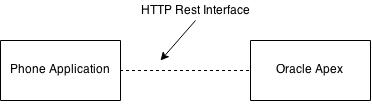
\includegraphics[width=0.5\textwidth]{diagrams/initialblockdiagram}
    \caption{Original design of the application}
    \label{fig:apex_block_diagram_image}
\end{figure} 

\subsubsection*{Functionality}

Assessing the functional requirements, required breaking down the concept into parts mainly posting, viewing and being notified about tags were the main parts to the functionality for the application.\\

%TODO:
%TALK ABOUT FUNCTIONALITY
%Viewing,
%Posting,
%Notifications

\subsubsection*{UI mock-ups}

Once the application had been broken down into the various functional areas I started to do some rough user interface layouts on paper, once they were to a satisfactory level they were converted into digital mock-ups using Balsamiq which created the figures \ref{fig:application_home_page_image}, \ref{fig:add_friend_activity_image}, \ref{fig:add_tag_activity_image}, \ref{fig:viewing_message_image}, \ref{fig:giving_friends_visability_image}, \ref{fig:login_activity_image}, \ref{fig:registration_activity_image} and \ref{fig:notification_image}. \\
\\
The UI design takes some inspiration from other phone applications in particular Snap Chat with the way of quickly sharing messages and Facebook with the quickly accessible stacked menu's, The main reason I took to take inspiration from Snap Chat is because there applications is very quick to use and post messages and the general concept of Lo Se Sono is almost the same bar we are using locations rather than pictures and there is no set timeout on the tags.\\
\\
At the time of creating the mock ups it was not clear at what platform the application was going to be implemented for, so the designs have remained very generic without being OS specific.\\
\\
These UI mock-ups were used to create the final application, the designs may have been slightly modified between the original design and the implementation in the final designs within the application.\\
\\
Figure \ref{fig:application_home_page_image} is the design for the main page of the application and what the users arrive on when the application launches so it is of up most important that this page is easy to navigate and informative to the user, the UI design has been intentionally designed to show the tags that are most relevant to the user at the time they have opened the application showing the tags in there immediate vicinity, theses can be either the users own tags or there friends who have left them there.\\

\begin{figure}[h!]
    \centering
    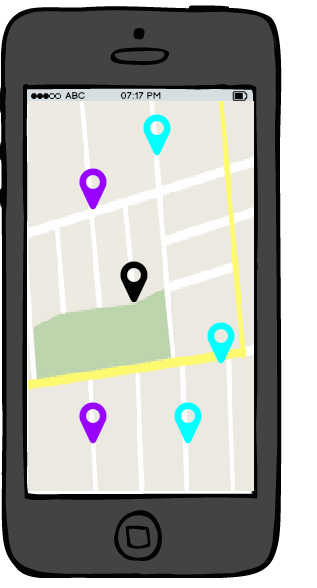
\includegraphics[width=0.25\textwidth]{uimockups/homepage}
    \caption{Application home page}
    \label{fig:application_home_page_image}
\end{figure}

\noindent
In figure \ref{fig:add_tag_activity_image} we are showing the initial design for adding a tag to the map, the key idea is to make it quick and easy to add a tag to the map and make it quickly accessible to the users friends so they can be promptly notified about the tag there friend has added.\\

\begin{figure}[h!]
    \centering
    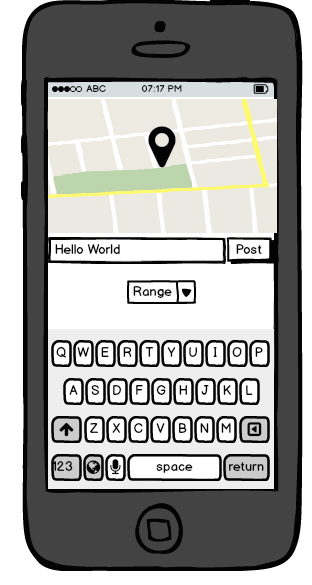
\includegraphics[width=0.25\textwidth]{uimockups/addtag}
    \caption{Adding a tag activity}
    \label{fig:add_tag_activity_image}
\end{figure}

\noindent
Pictured below in figure \ref{fig:giving_friends_visability_image} this is the screen that enables users friends to view a message that has been left, it should be relatively straight forward and easy to intemperate, the design has changed ever so slightly in the final implementation to try and make it fit in better with the Android design principles.\\

\begin{figure}[h!]
    \centering
    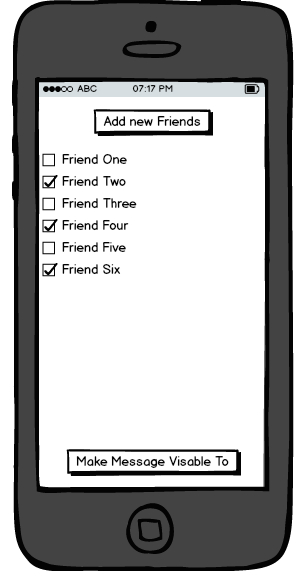
\includegraphics[width=0.25\textwidth]{uimockups/friendsvisability}
    \caption{Giving friends ability to view message}
    \label{fig:giving_friends_visability_image}
\end{figure} 

\noindent
This is the UI in figure \ref{fig:add_friend_activity_image} to add a new user to the users friends list it gives the user the ability to search for there friends using there names, in the final version of the application the search functionality remains unfinished within the UI but was partially completed within the server side application. When this functionality is implemented it should make it very easy for the user to add new friends within the application thus expanding the audience of the application.\\

\begin{figure}[h!]
    \centering
    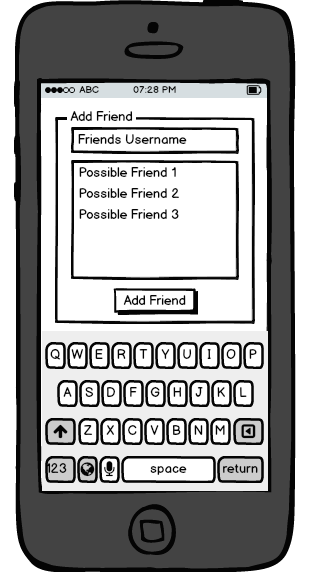
\includegraphics[width=0.25\textwidth]{uimockups/addfriend}
    \caption{Adding Friend activity}
    \label{fig:add_friend_activity_image}
\end{figure} 

\noindent
In this figure \ref{fig:viewing_message_image} we are show the viewing of a message, this is the screen that has changed the most from the original UI mock ups, where the icons and location of the voting section has been moved to be above the commenting area, there is also now a fixed area at the bottom for adding a comment along with each comment section now including there own voting sections, but again the changes to the initial designs intentionally have been very minor.\\

\begin{figure}[h!]
    \centering
    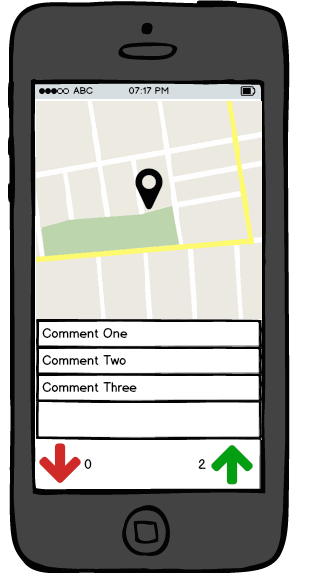
\includegraphics[width=0.25\textwidth]{uimockups/viewmessage}
    \caption{Viewing a message}
    \label{fig:viewing_message_image}
\end{figure} 

\noindent
The image below in figure \ref{fig:login_activity_image} shows the login screen for the application, this was intentionally kept simplistic to ensure that it is easy for the user to intemperate and should make it fairly secure against attacks as there are less fields to attack.\\

\begin{figure}[h!]
    \centering
    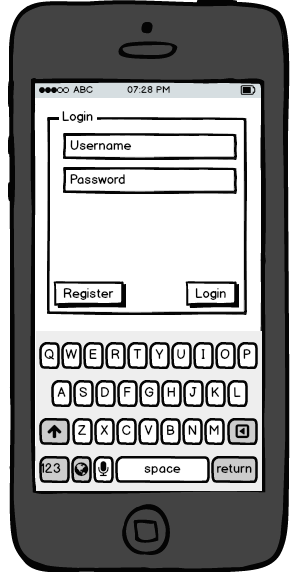
\includegraphics[width=0.25\textwidth]{uimockups/login}
    \caption{Login Activity for the application}
    \label{fig:login_activity_image}
\end{figure} 

\noindent
Screenshot pictured in figure \ref{fig:registration_activity_image} describes the registration page within the application that enables the user to register to use the application, again it has been kept simple to avoid confuse and ensure that the user can navigate it easily, this should easy annoyance when people are using the application for the first time.\\

\begin{figure}[h!]
    \centering
    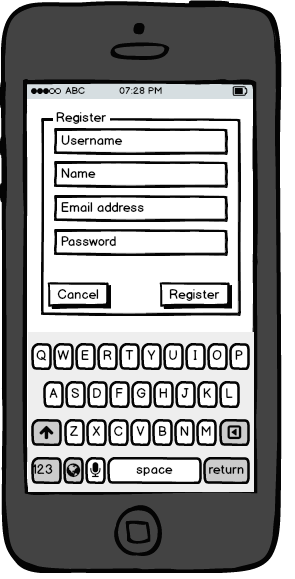
\includegraphics[width=0.25\textwidth]{uimockups/register}
    \caption{This is the activity for registering to use the application}
    \label{fig:registration_activity_image}
\end{figure} 

\noindent
This screenshot in figure \ref{fig:notificiation_image} is an example notification for the application, in the final application this does not look anything like this due to the fact we are using the Google Android notification API and notifications do not appear in this way.

\begin{figure}[h!]
    \centering
    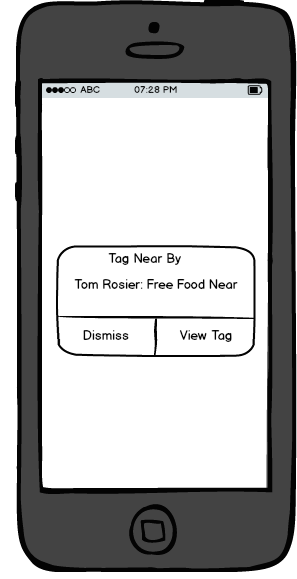
\includegraphics[width=0.25\textwidth]{uimockups/notification}
    \caption{Notification that there is a tag near by}
    \label{fig:notification_image}
\end{figure} 
\noindent


\subsection{Final Implementation}

{TODO}

\begin{figure}[h!]
    \centering
    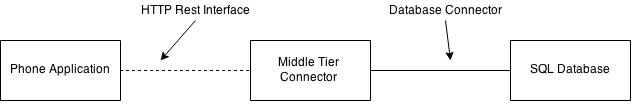
\includegraphics[width=\textwidth]{diagrams/blockdiagram}
    \caption{Very simple block diagram of the final architecture}
    \label{fig:final_block_diagram_image}
\end{figure} 
\noindent

\begin{figure}[h!]
    \centering
    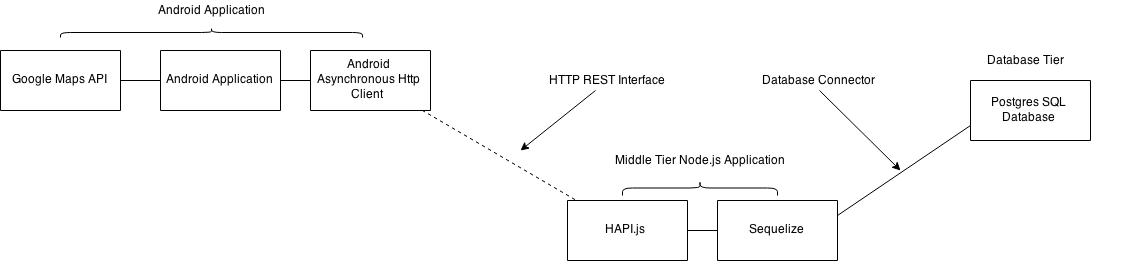
\includegraphics[width=\textwidth]{diagrams/finalblockdiagram}
    \caption{Very simple block diagram of the final architecture}
    \label{fig:final_block_diagram_image}
\end{figure} 
\noindent


\subsection{Future Development}

{TODO}

%Power considerations

%Scalability for different screen resolutions.

%Robust error handling.


\section{Client Side}

{TODO}

\subsection{Android Application}

{TODO}

\subsubsection*{Choice of Technologies}

{TODO}

\subsubsection*{Initial Design}

{TODO}

\subsubsection*{Application Structure}

{TODO}

\subsubsection*{Caveats}

{TODO}

% Talk about first time using android.



\section{Server Side}

{TODO}

\subsection{Middle Tier}

{TODO}

\subsubsection*{Choice of Technologies}

{TODO}

\subsubsection*{Rest interface}

{TODO}

\begin{figure}[h!]
    \centering
    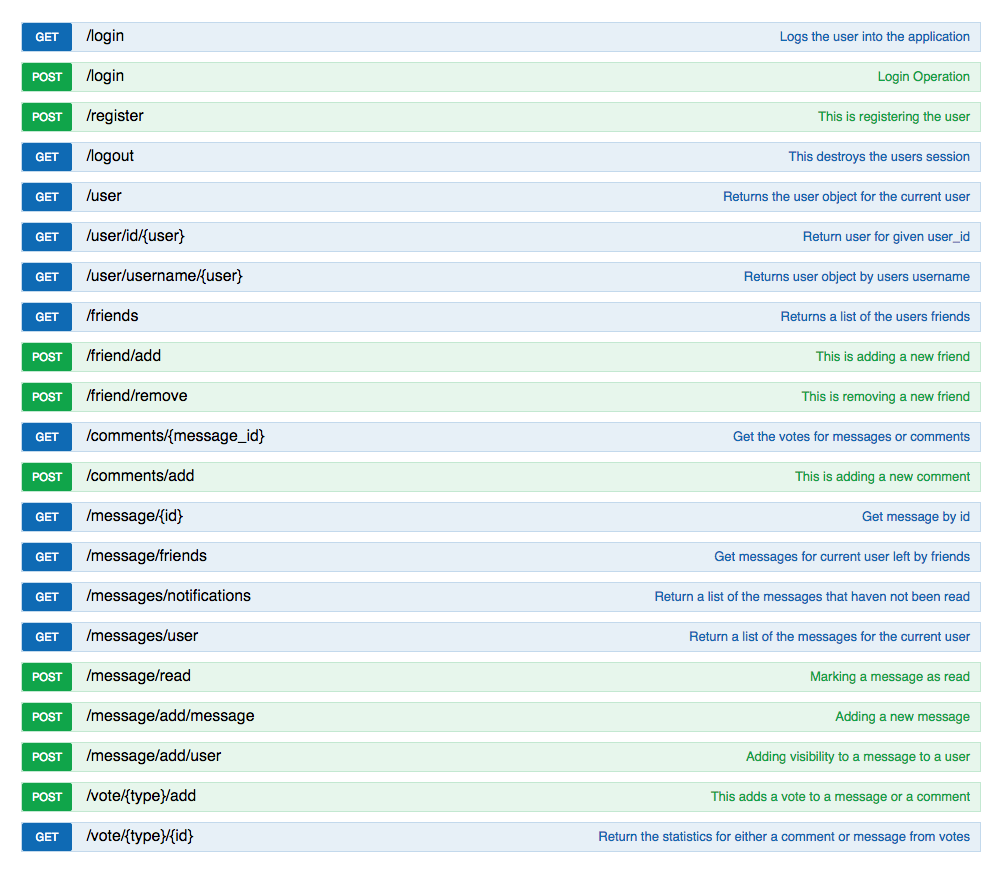
\includegraphics[width=\textwidth]{diagrams/restinterface}
    \caption{These are the endpoints for the REST API}
    \label{fig:rest_pai_diagram_image}
\end{figure} 
\noindent

\subsubsection*{Structure of application}

{TODO}

\subsubsection*{Authentication}

{TODO}

\subsection{Database level}

{TODO}

\subsubsection*{Choice of Technologies}

{TODO}

\subsubsection*{Database structure}

{TODO}

\begin{figure}[h!]
    \centering
    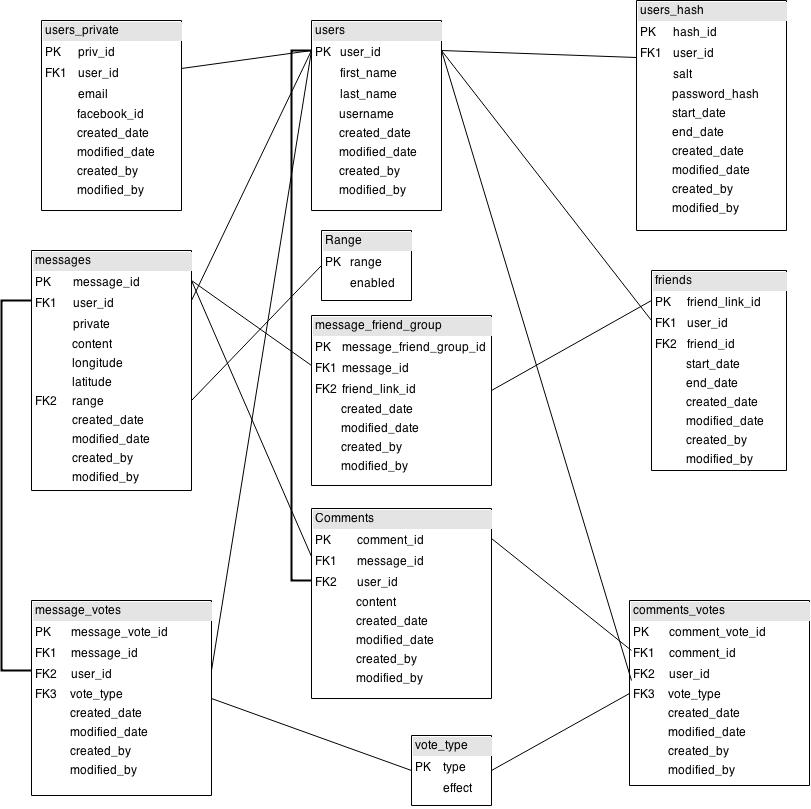
\includegraphics[width=\textwidth]{diagrams/database}
    \caption{This is the database design for the application}
    \label{fig:diagram_database_image}
\end{figure} 
\noindent

\subsubsection*{Alterations}

{TODO}

\subsubsection*{Protecting secrets}

{TODO}